\documentclass[10pt,preprint]{sigplanconf}
\usepackage{times}

\usepackage{datetime}
\usepackage{url}
\usepackage{hyperref}

\conferenceinfo{}{}
\copyrightyear{2017} 

\date{}

\authorinfo{}{}

\begin{document}

\title{Tuning Paxos for high-throughput with batching and pipelining} 
\maketitle

\section{Analytical model of Paxos performance}
\subsection{Quantitative analysis of Phase 2 of Paxos}
There are other variants of Paxos that use different communication schemes, like IP multicast and chained transmission in a ring. We chose the basic variant for generality and simplicity, but this analysis can be easily adapted to other variants. We assume full duplex links and that no other application is competing for bandwidth or CPU time. Also for simplicity, we focus on the best case, that is, do do not consider message loss or failures. We also ignore mechanisms internal to a full implementation of Paxos, like failure detection. On a finely tuned system, these mechanism should have a minimal impact on throughput. Finally, we assume that execution in each process is sequential. The model can be extended to account for multi-core or SMP machines, but this is not a non-trivial extension.

\begin{table}[h]
% \begin{table}[where]
% The argument 'where' specifies the allowed locations for the table.
% For example, when \begin{table}[h] is typed, it means that the
% table will appear on the top of the page.
\begin{center}
\begin{tabular}{l l} % 'l' is used for making the column contents left justified
Symbol & Description\\
\hline
$n$ & Number of replicas\\
$B$ & Bandwidth\\
$L$ & One way delay (latency)\\
$S_{req}$ & Size of request\\
$k$ & Number of requests in a batch\\
$w$ & Number of parallel instances\\
$S_{2a}$ & Size of a Phase 2a message (batch)\\
$S_{2b}$ & Size of ack\\
$S_{ans}$ & Size of answer sent to client\\
$\phi_{exec}$ & CPU-time used to execute a request\\
$WND$ & Bound on maximum number of parallel\\
      & instances (Configuration parameter)\\
$BSZ$ & Bound on batch size (Configuration parameter)
\end{tabular}
\vspace{-.1in} % vertical blank space
\end{center}
\caption{Notation.}
\label{tab:notation}
\end{table}

We focus on the two resources that are typically the bottleneck in a Paxos deployment, i.e., the leader's CPU and its outgoing channel.

For simplicity, we assume that all requests are of similar size. Since the bulk of Phase 2a message is the batch being proposed, in the following we use $S_{2a} = kS_{req} + c$ to denote the batch size, where $c$ represents the protocol headers.

\textbf{\emph{CPU time:}} During each instance, the leader uses the CPU to perform the following tasks: read the requests from the clients, prepare a batch containing $k$ requests, serialize and send $n - 1$ Phase 2a message, receive $n - 1$ Phase 2b messages, execute the requests and send the answers to the clients (in addition to executing the protocol logic whenever it receives a message).

These tasks can be divided in two categories: interaction with clients and with other replicas. The CPU time required to interact with clients depends mainly on the size of the requests ($S_{req}$) and the number of requests that must be read to fill a batch ($k$), while the interaction with replicas depends on the number of replicas ($n$) and the size of the batch ($S_{2a}$). Since these two interactions have distinct parameters and behaviors, we model them by two functions: $\phi_{cli}(x)$ and $\phi_{rep}(x)$. The function $\phi_{cli}(x)$ represents the CPU time used by the leader to receive a request from a clinet send back the corresponding answer, with $x$ being the sum of the sizes of the request and the answer. Similarly, $\phi_{rep}(x)$ is the CPU time used by the leader to interact with another replica, where $x$ is the sum of the sizes of the Phase 2a and 2b messages. Both functions are linear, which models the well-known behavior where the time to process a message consists of a constant plus a variable part, the later increasing linearly with the size of message.

Based on the previous discussion, we get the following expression for the CPU time of an instance:
\begin{multline}
T^{CPU}_{inst} = k\phi_{cli}(S_{req}+S_{ans}) \\
+(n-1)\phi_{rep}(S_{2a}+S_{2b})+k\phi_{exec}.
\end{multline}
% The multline environment is used to split one very long formula into several lines;
% the first is flushed left, the last is flushed right, and the middle lines are centered.
The first term models the cost of receiving $k$ requests from the clients and sending back the corresponding answers, the second item represents the cost of processing $n-1$ Phase 2a and 2b messages and, finally, the last term is the cost of executing $k$ requests.

\textbf{\emph{Wall-clock time:}} Estimating the wall-clock duration of an instance is challenging, because some operations that must complete for the instance to terminate are done in parallel. As an example, once the leader finishes sending $\lfloor n/2 \rfloor$ messages to the other replicas, the execution splits into two separate sequence of events. In one of them, the leader sends the remaining phase 2a messages. On the other, it waits for enough phase 2b messages to decide and start executing the requests. If after executing the first request in the batch, the leader did not finish sending all the Phase 2a messages, it may have to wait for the outgoing link to be free before sending the answers to the clients. Thus, the exact sequence that leads to completion depends on the workload and the characteristics of the system. In a fast LAN the wall-clock duration is likely to be limited by the CPU speed, while in a high-latency WAN the latency is likely the dominant factor. Similarly, if the workload consists of large requests and answers, the bandwidth is more likely to be the bottleneck than the CPU or the latency.

Therefore we model the wall-clock time by considering three different cases, each corresponding to a different bottleneck: CPU, bandwidth or latency. For each case, we compute the duration of an instance, which gives us three formulas: $T^{CPU}_{inst}$, $T^{band}_{inst}$,$T^{lat}_{inst}$.

For the LAN case, we have:
\begin{align}
T^{lat}_{inst} &= \lfloor n/2 \rfloor S_{2a}/B + 2L + k\phi_{exec} + kS_{ans}/B \label{inst:lat}
% & is a mark for the alignment point
%
% \begin{align}
% x_{k+1} & = x_k + \Phi(t_k, x_k) \nonumber \\
% & = x_k + h \cdot f(t_k, x_k) \\
% & = x_k + h \cdot \lambda \cdot e^{x_k}
% \end{align}
%
% \begin{align}
% f(x) &= g(x^2)\\
% a + b + c &= d + e + f
% \end{align}

\end{align}

\begin{figure}
\begin{center}
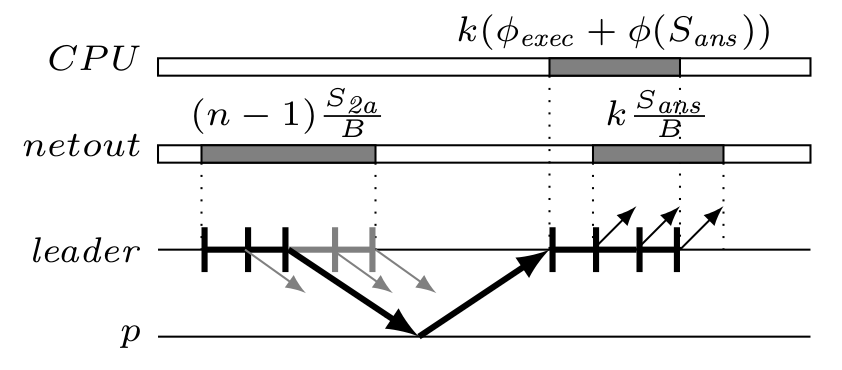
\includegraphics[width=.4\textwidth]{figures/wall-clock}
% width = length specifies the width to which the figure should be scaled.
% \textwidth - The horizontal extent of the text from left margin to right margin.
\end{center}
\caption{Utilization of the CPU and outgoing link of the leader during an instance.}
\label{fig:inst}
\end{figure}

Figure \ref{fig:inst} illustrates the three cases. Each sub-figure represents one instance. The two lines at the bottom represent the leader and the replica whose Phase 2b message triggers the decision at the leader. The two bars at the top represent the busy/idle periods of the CPU (\textbf{\emph{CPU time}}) and of the outgoing link of the leader. The arrows above the leader line represent messages exchanged with the clients and the arrows below are messages exchanged with the other replicas.

If the latency is the bottleneck (Equation \eqref{inst:lat}), the wall-clock time of an instance is the time needed to send the first $\lfloor n/2 \rfloor$ phase 2a messages to the replicas, plus the round-trip time required to receive enough Phase 2b messages from the replicas, followed by the execution of the request and the time to send the answers back to the clients.

\bibliographystyle{acm}
% \bibliography{xxx}

\end{document}


% LaTeX does not automatically word wrap
%
% \documentclass{article}
% \begin{document}
% \begin{table}
% \begin{tabular}{c|lll}
% Name&Salary&Likes&Children\\\hline
% Mark&$\$250,000$&windsurfing and jumping on trampolines&Amy, John, and Ray\\
% Carly&$\$80,000$&heavy metal music, Paris, and dancing in the rain&Tyra\\
% Carter&$\$25,000$&candy, fast cars that he cannot afford and Ramen&None\\
% Sam&$\$50,000$&painting, motorcycles, and Reddit&Kyle and Sam Jr.
% \end{tabular}
% \end{table}
% %%%%%%%%%%%%%%%%%%%%%%%%%%%%
% \begin{table}
% \begin{tabular}{c|lp{2in}p{1in}}
% Name&Salary&Likes&Children\\\hline
% Mark&$\$250,000$&windsurfing and jumping on trampolines&Amy, John, and Ray\\
% Carly&$\$80,000$&heavy metal music, Paris, and dancing in the rain&Tyra\\
% Carter&$\$25,000$&candy, fast cars that he cannot afford and Ramen&None\\
% Sam&$\$50,000$&painting, motorcycles, and Reddit&Kyle and Sam Jr.
% \end{tabular}
% \end{table}
% \end{document}
%
% We can see that this first table is not what we want since it overlaps the margins.
% Since we have not even included all the data we eventually want in the table, we
% need a way to fix this. We have one solution in the second table (which has the same
% information) where we force LaTeX to word wrap in individual cells by giving them a
% fixed width. The syntax for this is to use the justification character p followed by
% {width} where width is in some unit of length

% Cases constructions:
%
% \begin{equation}
% F_{n} = \begin{cases}
% 0 & \text{if $n = 0$;}\\
% 1 & \text{if $n = 1$;}\\
% F_{n - 1} + F_{n - 2} & \text{if $n > 0$.}
% \end{cases}
% \end{equation}
